% -*-latex-*-
% calculus.tex
%

\begin{section}{Formulas}
\begin{tabular}{l l}
  Quadratic Approximation & $f(u+x) ~= f(u) + f'(u) \cdot x + f''(u) \cdot x^2 / 2$\\
  $FTC2$ & $d/dx \int_0^x f(t) dt = f(x)$\\
  $FTC2$ Chain Rule & $d/dx \int_0^{g(x)} f(t) dt = g'(x) \cdot f(g(x))$ \\
  Weighted Average & $\int_a^b f(x) w(x) dx / \int_a^b w(x) dx$\\
\end{tabular}
\end{section}
\begin{section}{L'H\^opital's Rule}
  \[ \lim_{x \to a} f(x)/g(x) = \lim_{x \to a} f'(x)/g'(x) \]
  \begin{tabular}{l l}
    $0/0$&Straight up\\
    $\infty/\infty$&Straight up\\
    $0 \cdot \infty$ & Rewrite as quotient\\
    $0^0$& Rewrite as $e^{ln(f)}$ \\
    $\infty^0$& Rewrite as $e^{ln(f)}$ \\
    $1^\infty$& Rewrite as $e^{ln(f)}$ \\
    $\infty - \infty$&Good luck \\
    Otherwise & Forget it. \\
  \end{tabular}

\end{section}

\begin{section}{Vector Products}
  \begin{subsection}{Dot Product}
    \begin{figure}[h!]
      \begin{center}
        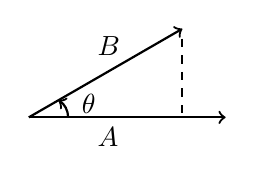
\begin{tikzpicture}[scale=0.5]
          \draw [thick, ->] (0,0) to (5,0);
          \draw [thick, ->] (0,0) to (3.9,2.25);
          \draw [thick,dashed] (3.9,2.0) to (3.9,0);
          \draw [thick, ->] (1,0) arc
          [start angle=0, end angle=60, radius=0.5];
          \draw [fill] (1.5,1.8) node [black,right] {$B$};
          \draw [fill] (1.5,-0.5) node [black,right] {$A$};
          \draw [fill] (1.1,0.35) node [black,right] {$\theta$};
        \end{tikzpicture}
        \caption{Dot Product}
      \end{center}
    \end{figure}
    $\vec{A}\cdot\vec{B} =
    \left|\vec{A}\right|\left|\vec{B}\right|cos(\theta)$

    The scalar value of the dot product is the sum of the product of
    the vector components $\Sigma\, a_i \cdot b_i$

    Geometrically, the scalar value is the length of the projection of
    $\vec{B}$ onto $\vec{A}$.
    \FloatBarrier
  \end{subsection}

  \begin{subsection}{Cross Product}
    \begin{figure}[h!]
      \begin{center}
        \begin{tikzpicture}[scale=0.5]
          \begin{scope}[canvas is xy plane at z=0]
            \draw [->] (-2,1) to (-1,1);
            \draw [fill] (-1,1) node [black,right] {$x$};
            \draw [->] (-2,1) to (-2,2);
            \draw [fill] (-2.5,2.5) node [black,right] {$y$};
            \draw [thick, ->] (0,0) to (5,0);
            \draw [thick, ->] (0,0) to (3.9,2.25);
            \draw [thick,dashed,->] (3.9,2.25) to (8.6,2.25);
            \draw [thick,dashed,->] (5,0) to (8.9,2.25);
            \draw [thick, ->] (1,0) arc
            [start angle=0, end angle=60, radius=0.5];
            \draw [fill] (1.5,1.8) node [black,right] {$B$};
            \draw [fill] (1.5,-0.5) node [black,right] {$A$};
            \draw [fill] (1.1,0.35) node [black,right] {$\theta$};
            \draw[help lines] (0,0) grid (10,3);
          \end{scope}
          \begin{scope}[canvas is zx plane at y=0]
            \draw [thick, ->] (0,0) to (8.775,0);
            \draw [fill] (8.8,0) node [black,right] {$\hat{n}$};
          \end{scope}
          \begin{scope}[canvas is zx plane at y=1]
            \draw [->] (0,-2) to (1,-2);
            \draw [fill] (1.5,-2.7) node [black,right] {$z$};
          \end{scope}
        \end{tikzpicture}
        \caption{Cross Product}
      \end{center}
    \end{figure}
    $\vec{A}\times\vec{B} =
    \left|\vec{A}\right|\left|\vec{B}\right|sin(\theta)\hat{n}$

    Geometrically, the vector value of the cross product is the area
    of the parallelogram formed by $\vec{B}$ and $\vec{A}$ times the
    unit vector $\hat{n}$ normal to the plane of the parallelogram
    following the right hand rule.

    \FloatBarrier

  \end{subsection}
  \begin{subsection}{Special Values}
    \begin{align*}
      \vec{A}\cdot\vec{B} &>0&&\theta \text{ is acute.} \\
      \vec{A}\cdot\vec{B} &<0&&\theta \text{ is obtuse.} \\
      \vec{A}\cdot\vec{B} &=0&&\text{Vectors are orthogonal.} \\
      \vec{A}\times\vec{B} &=0&&\text{Vectors are parallel.} \\
    \end{align*}

  \end{subsection}

\end{section}


\begin{section}{Parametric Vector Calculus}
  \begin{tabular}{l l l l l l}
    Position & & & $\vec{r}(t)=x(t)\hat{i}+y(t)\hat{j}$  & $\int \vec{v}(t) dt$ &\\
    Velocity & $d\vec{r}(t)/dt$ & & $\vec{v}(t)=x'(t)\hat{i}+y'(t)\hat{j}$ &  $\int \vec{a}(t) dt$& $\frac{ds}{dt} \vec{T}$\\
    Acceleration & $d\vec{v}(t)/dt$ & $d^2\vec{r}(t)/dt^2$ & $\vec{v}(t)=x''(t)\hat{i}+y''(t)\hat{j}$ & &\\
    Arc Length & $\frac{ds}{dt} = \sqrt{x'(t)\hat{i}+y'(t)\hat{j}}$  & & & & \\
    Unit Tangent & $\hat{T}=\vec{v}/\left| \vec{v} \right|$ &&&&
  \end{tabular}

\end{section}
\begin{section}{Partial Differentiation}
  \begin{tabular}{l l}
    Tangent Plane to $f(x_{0},y_{0})$ & \begin{math}
      z-z_0 =(\frac{\partial{f}}{\partial{x}})_{x_{0}}(x-x_0) + (\frac{\partial{f}}{\partial{y}})_{y_{0}}(y-y_0)
      \end{math} \\
    Approximation & $f(x,y)=z_0 + \frac{\partial{f}}{\partial{x}}(x-x_0) + \frac{\partial{f}}{\partial{y}}(y-y_0)$ \\

  \end{tabular}
  % lwarp seems to have problems with this construct in the table above.
  \begin{section}{Least Square Line}
    \begin{math}
      \begin{pmatrix}
        \sum x_i^2 & \sum x_i \\
        \sum x_i & n \\
      \end{pmatrix}^{-1}
      \begin{pmatrix}
        \sum x_i y_i \\
        \sum y_i \\
      \end{pmatrix}
      =
      \begin{pmatrix}
        a \\
        b \\
      \end{pmatrix}
    \end{math}
    for $y = ax + b$ given $n$ points $(x_i,y_i)$
  \end{section}
  \begin{section}{Second Derivative Test}
    Given $f(x,y)$ critical points $(x_c,y_c)$ where $\frac{\partial{f}}{\partial{x}}=0$ and  $\frac{\partial{f}}{\partial{y}}=0$

    \begin{tabular}{l}
      $A = \frac{\partial^2{f}}{\partial{x}^2}@(x_c,y_c)$ \\
      $B = \frac{\partial^2{f}}{\partial{x}\partial{y}}@(x_c,y_c)$ \\
      $C = \frac{\partial^2{f}}{\partial{y}^2}@(x_c,y_c)$ \\
    \end{tabular}

    \begin{tabular}{l l}
      $AC-B^2 > 0$ , $A>0$ or $C>0$  & Minimum point \\
      $AC-B^2 > 0$ , $A<0$ or $C<0$  & Maximum point \\
      $AC-B^2 < 0$  & Saddle point \\
      $AC-B^2 = 0$  & Need higher order terms to conclude \\
    \end{tabular}

  \end{section}
  \begin{section}{Differential Chain Rule}
    $f(x(t),y(t),z(t))$;
    $\frac{df}{dt}=
    f_{x}\frac{dx}{dt} + f_{y}\frac{dy}{dt} + f_{z}\frac{dz}{dt}$
  \end{section}

  \begin{section}{Level Curves and Surfaces}
    The \emph{level curve} for a function $f(x,y)$ is the set of
    points $(x,y)$ where $f(x,y)=C$ for constant $C$.
  \end{section}

  \begin{section}{Gradient}
    The \emph{gradient} $\nabla{f}$ of (\emph{potential})
    function $f$ is a vector of the
    partial derivatives of $f$ for each independant variable; e.g.
    $\nabla f(x,y) = \langle f_x,f_y \rangle $.
    $\nabla{f} \perp f(x,y)$, i.e.  \emph{gradient} $\perp$
    \emph{level curve}.

    The \emph{directional derivitive} of $f$ at the point $P$ in the
    direction of $\vec{u}$ is
    $\frac{df}{ds}\biggr\rvert_{P,\vec{u}}=\nabla{f}(P)\cdot\vec{u}$.

    Given an \emph{objective} function $f$ and a \emph{constraint}
    function $g=C$ for constant $C$, the \emph{extrema} of $f$
    are found when $\nabla{f} \parallel \nabla{g}$. The
    \emph{Lagrange multiplier} $\lambda$ is
    $\frac{\nabla{f}}{\nabla{g}}$.
  \end{section}
  \begin{section}{Center of Mass}
    \begin{tabular}{l l}
      $M$ & Mass\\
      $\delta$ & Density Function\\
      $\bar{x}$ & $x$ center\\
      $\bar{y}$ & $y$ center\\
    \end{tabular}
    \begin{align*}
      M&=\int\int_R{\delta} \,dA\\
      \bar{x}&=\frac{1}{M}\int\int_R{x\delta} \,dA\\
      \bar{y}&=\frac{1}{M}\int\int_R{y\delta} \,dA\\
    \end{align*}
  \end{section}

  \begin{section}{Moment of Inertia}
    \begin{tabular}{l l}
      $I_x$ & Moment about $x$ axis \\
      $I_y$ & Moment about $y$ axis \\
    \end{tabular}
    \begin{align*}
      I_x&=\int\int_R{\delta}y^2 \,dy\\
      I_y&=\int\int_R{\delta}x^2 \,dx\\
    \end{align*}
  \end{section}

  \begin{section}{Change of Variables}
    \begin{align*}
      \int\int_R{f(x,y) \,dx \,dy} &=\int\int_R{g(u,v)\, |J| \,du \,dv} \\
      g(u,v) &= f(x(u,v),y(u,v)) \\
      |J| &=
            \begin{vmatrix}
              \frac{\partial{(x,y)}}{\partial{(u,v)}}\\
            \end{vmatrix} =
      \begin{vmatrix}
        \frac{\partial{x}}{\partial{u}} & \frac{\partial{x}}{\partial{v}}\\
        \frac{\partial{y}}{\partial{u}} & \frac{\partial{y}}{\partial{v}}\\
      \end{vmatrix} \\
      \begin{vmatrix}
        \frac{\partial{(x,y)}}{\partial{(u,v)}}\\
      \end{vmatrix}
      \cdot
      \begin{vmatrix}
        \frac{\partial{(u,v)}}{\partial{(x,y)}}
      \end{vmatrix}
      &= 1
    \end{align*}
  \end{section}

  \begin{section}{Vector Field}
    \begin{tabular}{l l l}
     $\vec{F}$ & Field & \\
     $M$ & Field component in $x$ direction ($\hat{i}$) & $F_x$ \\
     $N$ & Field component in $y$ direction ($\hat{j}$) & $F_y$ \\
     $C$ & Curve $\vec{r}(t)$ = $ \langle x(t),y(t) \rangle $ & \\
    \end{tabular}
    \begin{align*}
      \vec{F}(x,y) &= \langle M,N \rangle \\
      \vec{F}(x,y) &= M(x,y)\hat{i} + N(x,y)\hat{j}\\
      \text{curl}\,\vec{F} &= N_x - M_y  \\
      \text{div}\,\vec{F} &= M_x + N_y  \\
    \end{align*}
  \end{section}

  \begin{section}{Rectangular/Polar Conversion}
    \begin{align*}
      x &= r\,cos(\theta) \\
      y &= r\,sin(\theta) \\
      \theta &= tan^{-1}(y/x) \\
      r &= \sqrt{x^2+y^2} \\
      dx\,dy &= r\,dr\,d\theta\\
    \end{align*}
  \end{section}

  \begin{section}{Complex Arithmetic}
    \begin{align*}
      i &= \sqrt{-1} && \text{Imaginary unit} \\
      z &= a + bi && \text{Complex number z} \\
      \bar{z} &= a - bi && \text{Complex congugate} \\
      a &= Re(a + bi) &&  \text{Real part} \\
      b &= Im(a + bi) && \text{Imaginary part} \\
      (a+bi)+(c+di) &= (a+c) + (b+d)i && \text{Addition} \\
      (a+bi)\cdot(c+di) &= (ac-bd) + (ad+bc)i && \text{Multiplication} \\
      \frac{a+bi}{c+di} &= \frac{(ac+bd) + (bc-ad)i}{c^2+d^2} && \text{Division} \\
      \abs{z} &= \sqrt{a^2+b^2} && \text{Absolute value, Modulus} \\
      arg(z) &= tan^{-1}(b/a) = \theta && \text{Argument} \\
      z\bar{z} &= \abs{z}^2 && \text{Modulus squared} \\
      e^{i\theta} &= cos(\theta) + i\,sin(\theta) && \text{Euler's Formula} \\
      z &= \abs{z}[cos(\theta) + i\,sin(\theta)] && \text{Polar form I} \\
      z &= \abs{z}e^{i\theta} && \text{Polar form II} \\
    \end{align*}
  \end{section}

  \begin{section}{Sinusoidal Functions}
    \begin{tabular}{l l}
      $A$ & Amplitude \\
      $\omega$ & Angular Frequency\\
      $\phi$ &Phase lag \\
      $\tau$ & Time delay \\
      $\nu$ & Frequency \\
      $P$ & Period \\
    \end{tabular}
    \begin{align*}
      f(t) &= A\,cos(\omega\,t - \phi) \\
      f(t) &= A\,cos(\omega\,(t - \tau)) \\
      \tau &= \phi / \omega \\
      \nu &= \omega / 2\pi \\
      P &= 1/\nu \\
    \end{align*}
  \end{section}

  \begin{section}{Sinusoidal Identity}
    \begin{align*}
      a\,cos(\omega\,t)+b\,cos(\omega\,t) &= A\,cos(\omega\,t - \phi)
    \end{align*}

    \begin{tabular}{l l}
      $a\,cos(\omega\,t)+b\,cos(\omega\,t)$ & Rectangular (Cartesian) form \\
      $A\,cos(\omega\,t - \phi)$ & Amplitude-phase form \\
    \end{tabular}

    \begin{align*}
      A &= \sqrt{a^2+b^2} \\
      \phi &= tan^{-1}(b/a) \\
      a+bi &= Ae^{i\phi} \\
      a &= A\,cos(\phi) \\
      b &= A\,sin(\phi)
    \end{align*}
    \begin{figure}[h!]
      \begin{center}
        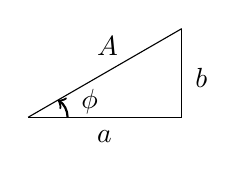
\begin{tikzpicture}[scale=0.5]
          \draw (0,0) to (3.9,0);
          \draw (0,0) to (3.9,2.25);
          \draw (3.9,2.25) to (3.9,0);
          \draw [thick, ->] (1,0) arc
          [start angle=0, end angle=60, radius=0.5];
          \draw [fill] (1.5,1.8) node [black,right] {$A$};
          \draw [fill] (1.5,-0.5) node [black,right] {$a$};
          \draw [fill] (4.0,1.0) node [black,right] {$b$};
          \draw [fill] (1.1,0.4) node [black,right] {$\phi$};
        \end{tikzpicture}
        \caption{$a+bi=Ae^{i\phi}$}
      \end{center}
    \end{figure}
  \end{section}

  \begin{section}{Line Integral}
    \begin{align*}
      C &=\vec{r}(t) \\
      s &= \text{arc-length}(C) \\
      \vec{r}(t) &=\langle x(t),y(t) \rangle  \\
      P(t) &= M(x,y) \\
      Q(t) &= N(x,y) \\
    \end{align*}
    \begin{subsection}{Work}
      Force on particle along a curve.
      \begin{figure}[h!]
        \begin{center}
          \begin{tikzpicture}
            % x = 23*t^3 - 33*t^2 + 18*t + 1
            % y = 22*t^3 - 33*t^2 + 12*t + 2
            \draw (1,2) .. controls (7,6) and (2,-1) .. (9,3);
            \draw (0,0) to (0,4);
            \draw (0,0) to (9,0);
            \draw [->] (0,0) to (3.464, 3.256); %t= 0.2
            % \draw (2,2.977) to (5,3.549); % tangent line at t=0.2
            \draw [->] (3.464, 3.256) to (4.446,3.443); % tangent unit vector
            \draw [->] (3.464, 3.256) to (4.464, 2.256); % force vector
            \draw [fill] (1.0,2.0) node [black,left] {$C$};
            \draw [fill] (2.0,2.8) node [black,left] {$s$};
            \draw [fill] (0.7,0.5) node [black,right] {$\vec{r}$};
            \draw [fill] (4.3,1.9) node [black,right] {$\vec{F}$};
            \draw [fill] (4.5,3.5) node [black,right] {$\hat{T}$};
          \end{tikzpicture}
          \caption{Work}
        \end{center}
      \end{figure}
      \begin{align*}
        \int_C \vec{F} \cdot d\vec{r} &= \int_C \vec{F} \cdot \hat{T} \, ds \\
                                      &= \int_C \langle M,N \rangle \cdot \langle dx,dy \rangle \\
                                      &= \int_C M\,dx + N\,dy \\
                                      &= \int_C (P + Q) \,dt \\
      \end{align*}
      \FloatBarrier
    \end{subsection} % Work
    \begin{subsection}{Flow}
      Flow across a curve.
      \begin{figure}[h!]
        \begin{center}
          \begin{tikzpicture}
            % x = 23*t^3 - 33*t^2 + 18*t + 1
            % y = 22*t^3 - 33*t^2 + 12*t + 2
            \draw (1,2) .. controls (7,6) and (2,-1) .. (9,3);
            \draw (0,0) to (0,4);
            \draw (0,0) to (9,0);
            \draw [->] (0,0) to (3.464, 3.256); %t= 0.2
            % \draw (2,2.977) to (5,3.549); % tangent line at t=0.2
            \draw [->] (3.464, 3.256) to (3.651, 2.274); % normal unit vector
            \draw [->] (3.464, 3.256) to (4.464, 2.256); % force vector
            \draw [fill] (1.0,2.0) node [black,left] {$C$};
            \draw [fill] (2.0,2.8) node [black,left] {$s$};
            \draw [fill] (0.7,0.5) node [black,right] {$\vec{r}$};
            \draw [fill] (4.3,1.9) node [black,right] {$\vec{F}$};
            \draw [fill] (3.6,2.2) node [black,right] {$\hat{n}$};
          \end{tikzpicture}
          \caption{Flow}
        \end{center}
      \end{figure}
      \begin{align*}
        \int_C \vec{F}\cdot\hat{n}\,ds
                                      &= \int_C \langle M,N \rangle \cdot \langle dy,-dx \rangle \\
                                      &= \int_C -N\,dx + M\,dy \\
                                      &= \int_C (P - Q) \,dt \\
      \end{align*}
      \FloatBarrier
    \end{subsection} % Flow
    \begin{subsection}{Area}
      Area of a simply connected closed curve.
      %% Need picture
      \begin{align*}
        A &= \frac{1}{2} \oint_C -y\,dx + x\,dy \\
      \end{align*}
      \FloatBarrier
    \end{subsection} % Area
  \end{section}

  \begin{section}{Gradient Field}

    If $\vec{F}(x,y) == \nabla{f}$
    then the field $\vec{F}$ is \emph{conservative}.

    \begin{align*}
      \int_a^b \vec{F} \cdot d\vec{r} &= f(b) - f(a) &&
      \text{Fundamental Theorem for Line Integrals}\\
      \int_{C_1} \vec{F} \cdot d\vec{r} &= \int_{C_2} \vec{F} \cdot d\vec{r} &&
      \text{Path independence}\\
      \oint \vec{F} \cdot d\vec{r} &= 0 &&
      \text{If $\vec{r}$ is a closed path}\\
    \end{align*}
  \end{section}

  \begin{section}{Green's Theorem}
    \begin{align*}
      \oint_C \vec{F} \cdot d\vec{r} &= \int\int_R curl(\vec{F})\,dA && \text{tangental} \\
      \oint_C \vec{F} \cdot \hat{n}\, ds &= \int\int_R div(\vec{F})\,dA && \text{normal} \\
    \end{align*}
  \end{section}

% TODO: Potential Functions

%  \begin{section}{}
%    \begin{tabular}{l l}
%      &  \\
%   \end{tabular}
%    \begin{align*}
%      &=\\
%    \end{align*}
%  \end{section}

\end{section}
